\documentclass{beamer} 
\usepackage{amsmath,amsthm}
\usepackage{graphicx,microtype,parskip}
\usepackage{caption,subcaption,multirow}
\usepackage{attrib}

\frenchspacing

\usetheme{Berlin}
\usecolortheme{beaver}

\setbeamertemplate{navigation symbols}{}

\setbeamercolor{title}{fg=red,bg=white}

\setbeamercolor{block title}{fg=white,bg=gray}
\setbeamercolor{block body}{fg=black,bg=lightgray}

\setbeamercolor{block title alerted}{fg=white,bg=darkgray}
\setbeamercolor{block body alerted}{fg=black,bg=lightgray}

%\AtBeginSection[]
%{
%  \begin{frame}
%    \tableofcontents[currentsection]
%  \end{frame}
%}

\title{The Roof is on Fire}
\subtitle{The flammability of the Darwin cluster}
\author{Peter D Smits}
\institute{Committee on Evolutionary Biology, University of Chicago}
\date{}

\begin{document}

\begin{frame}
  \maketitle
\end{frame}

\begin{frame}
  \begin{center}
    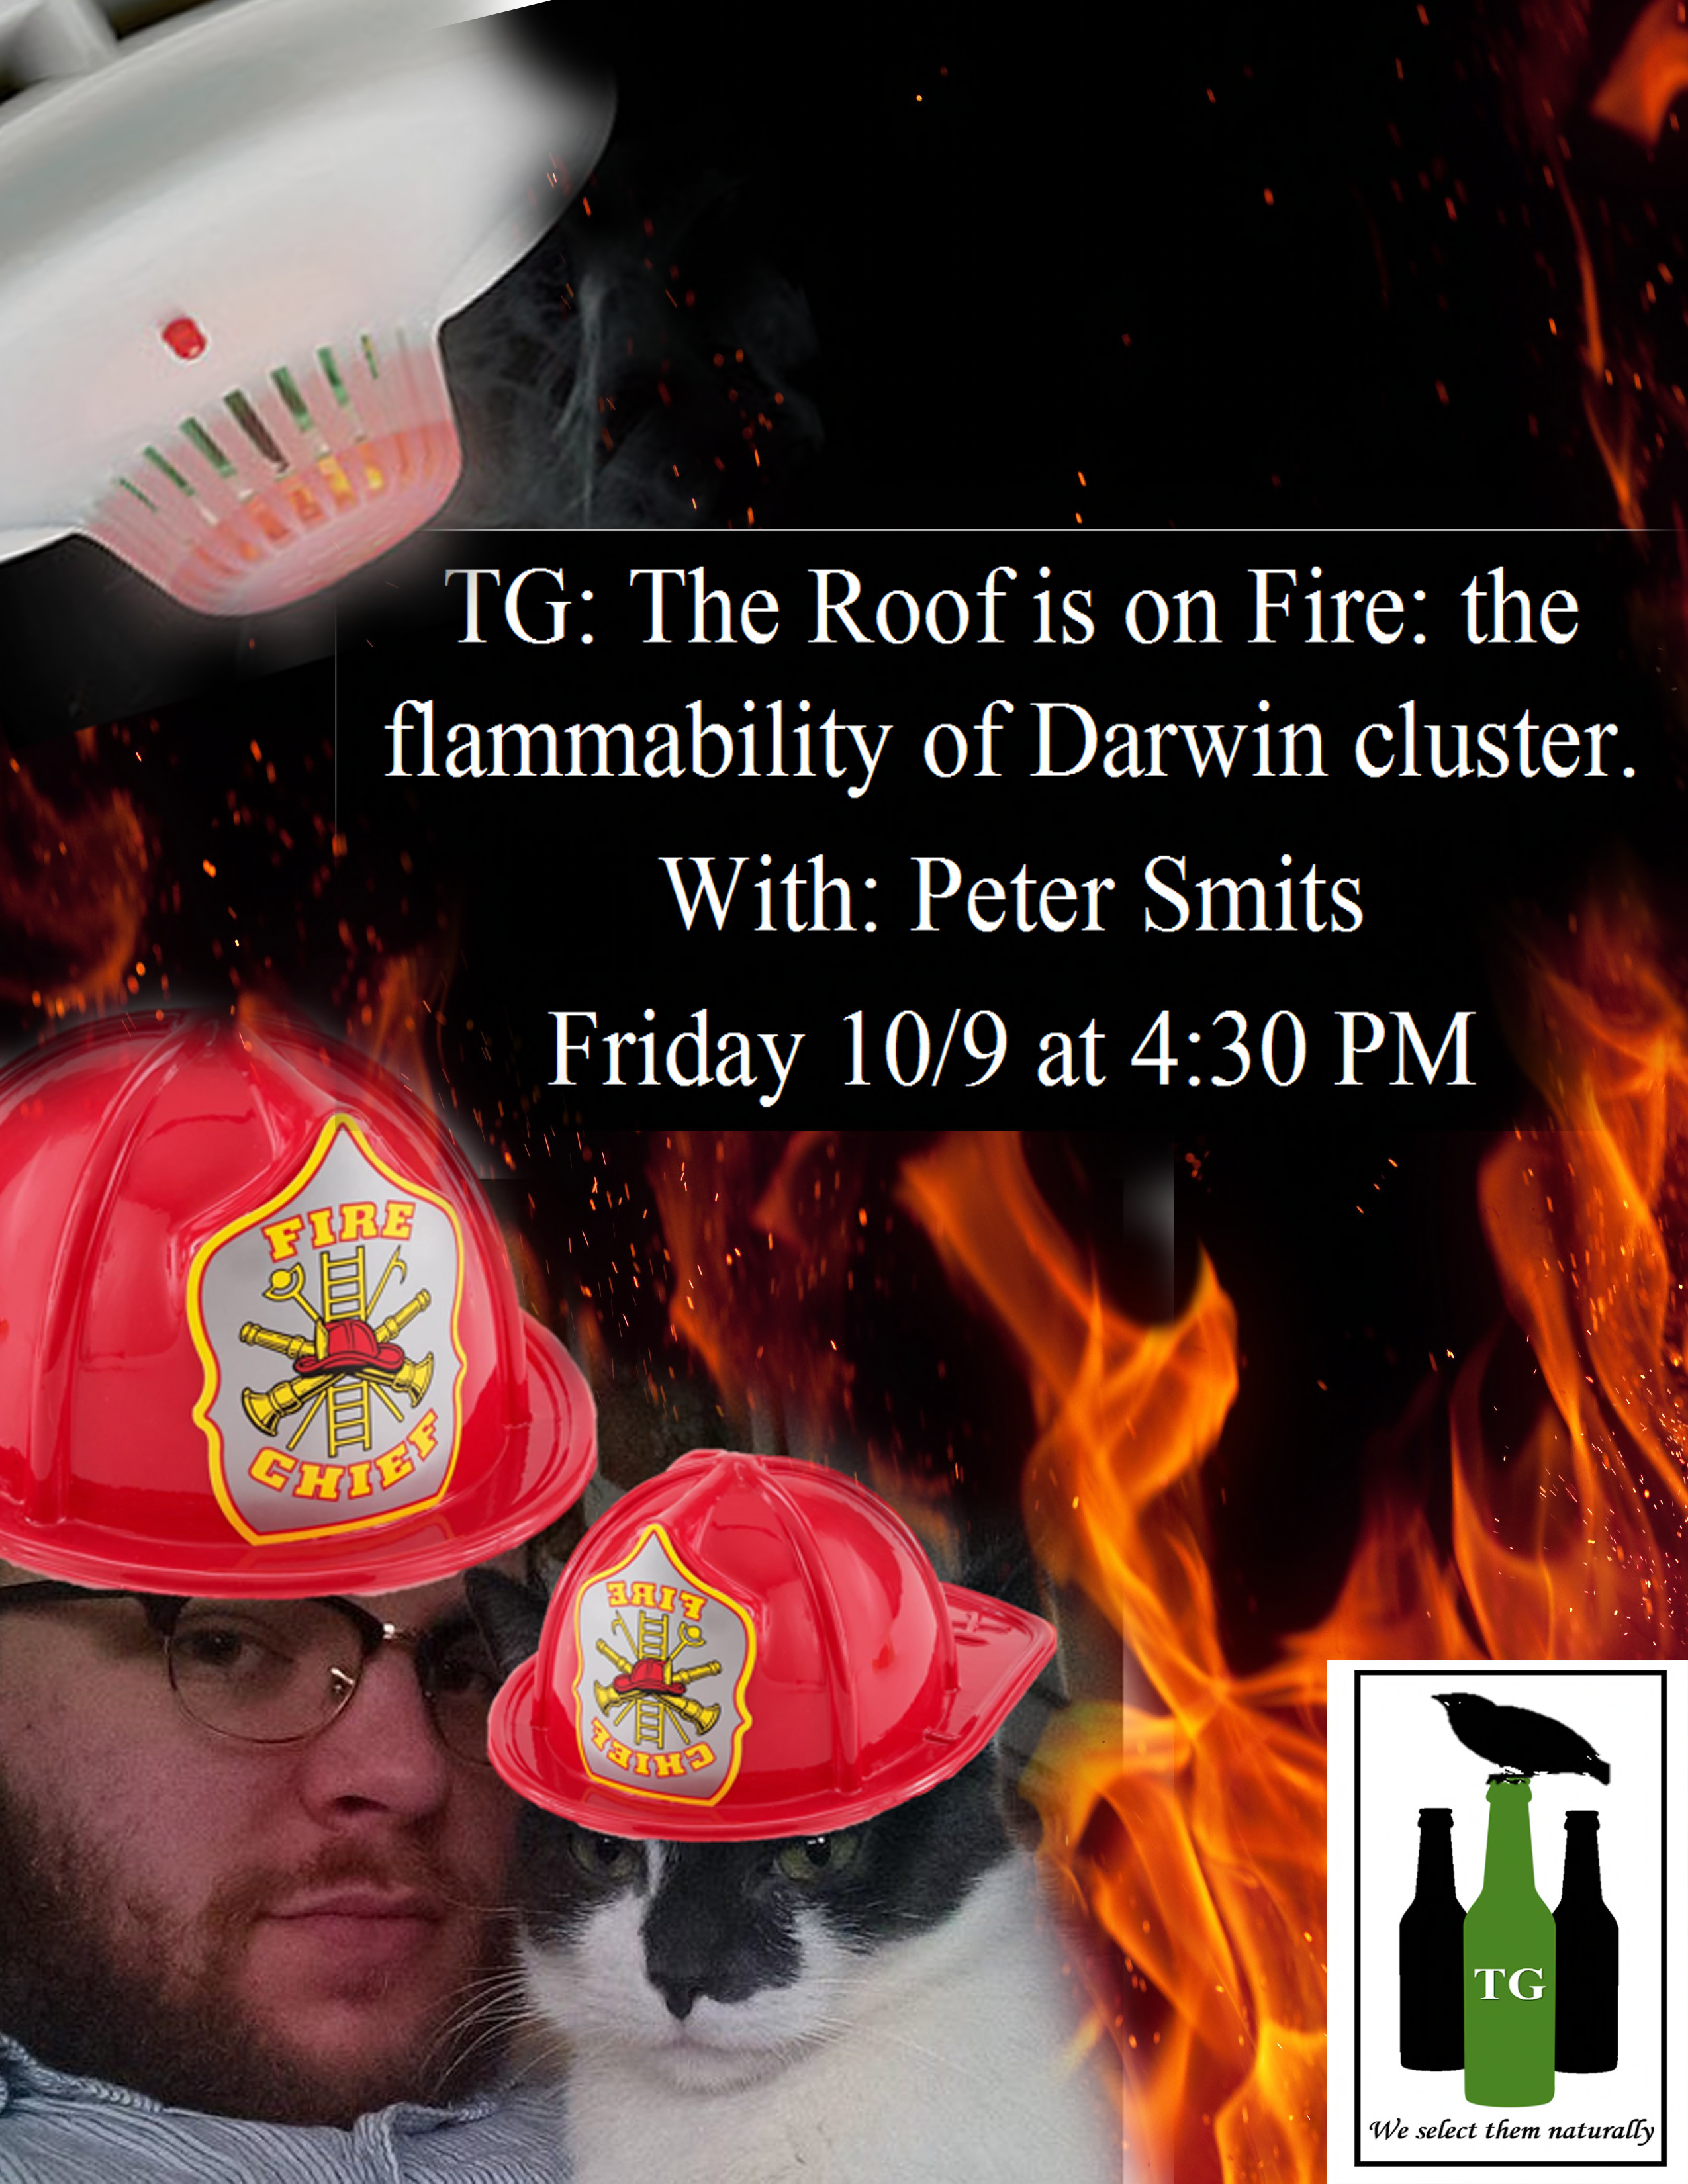
\includegraphics[width=\textwidth,height=0.8\textheight,keepaspectratio=true]{TGposter1}
  \end{center}
\end{frame}

\begin{frame}
  \begin{center}
    
\includegraphics[width=\textwidth,height=0.8\textheight,keepaspectratio=true]{chicago_flag}
  \end{center}
\end{frame}

\begin{frame}
  \begin{center}
    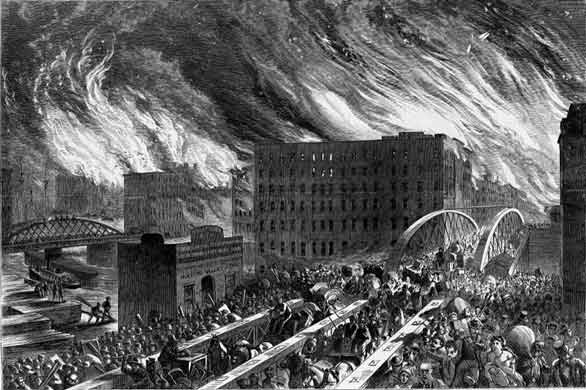
\includegraphics[width=\textwidth,height=0.8\textheight,keepaspectratio=true]{chicago_fire_1}
  \end{center}
\end{frame}

\begin{frame}
  \begin{center}
    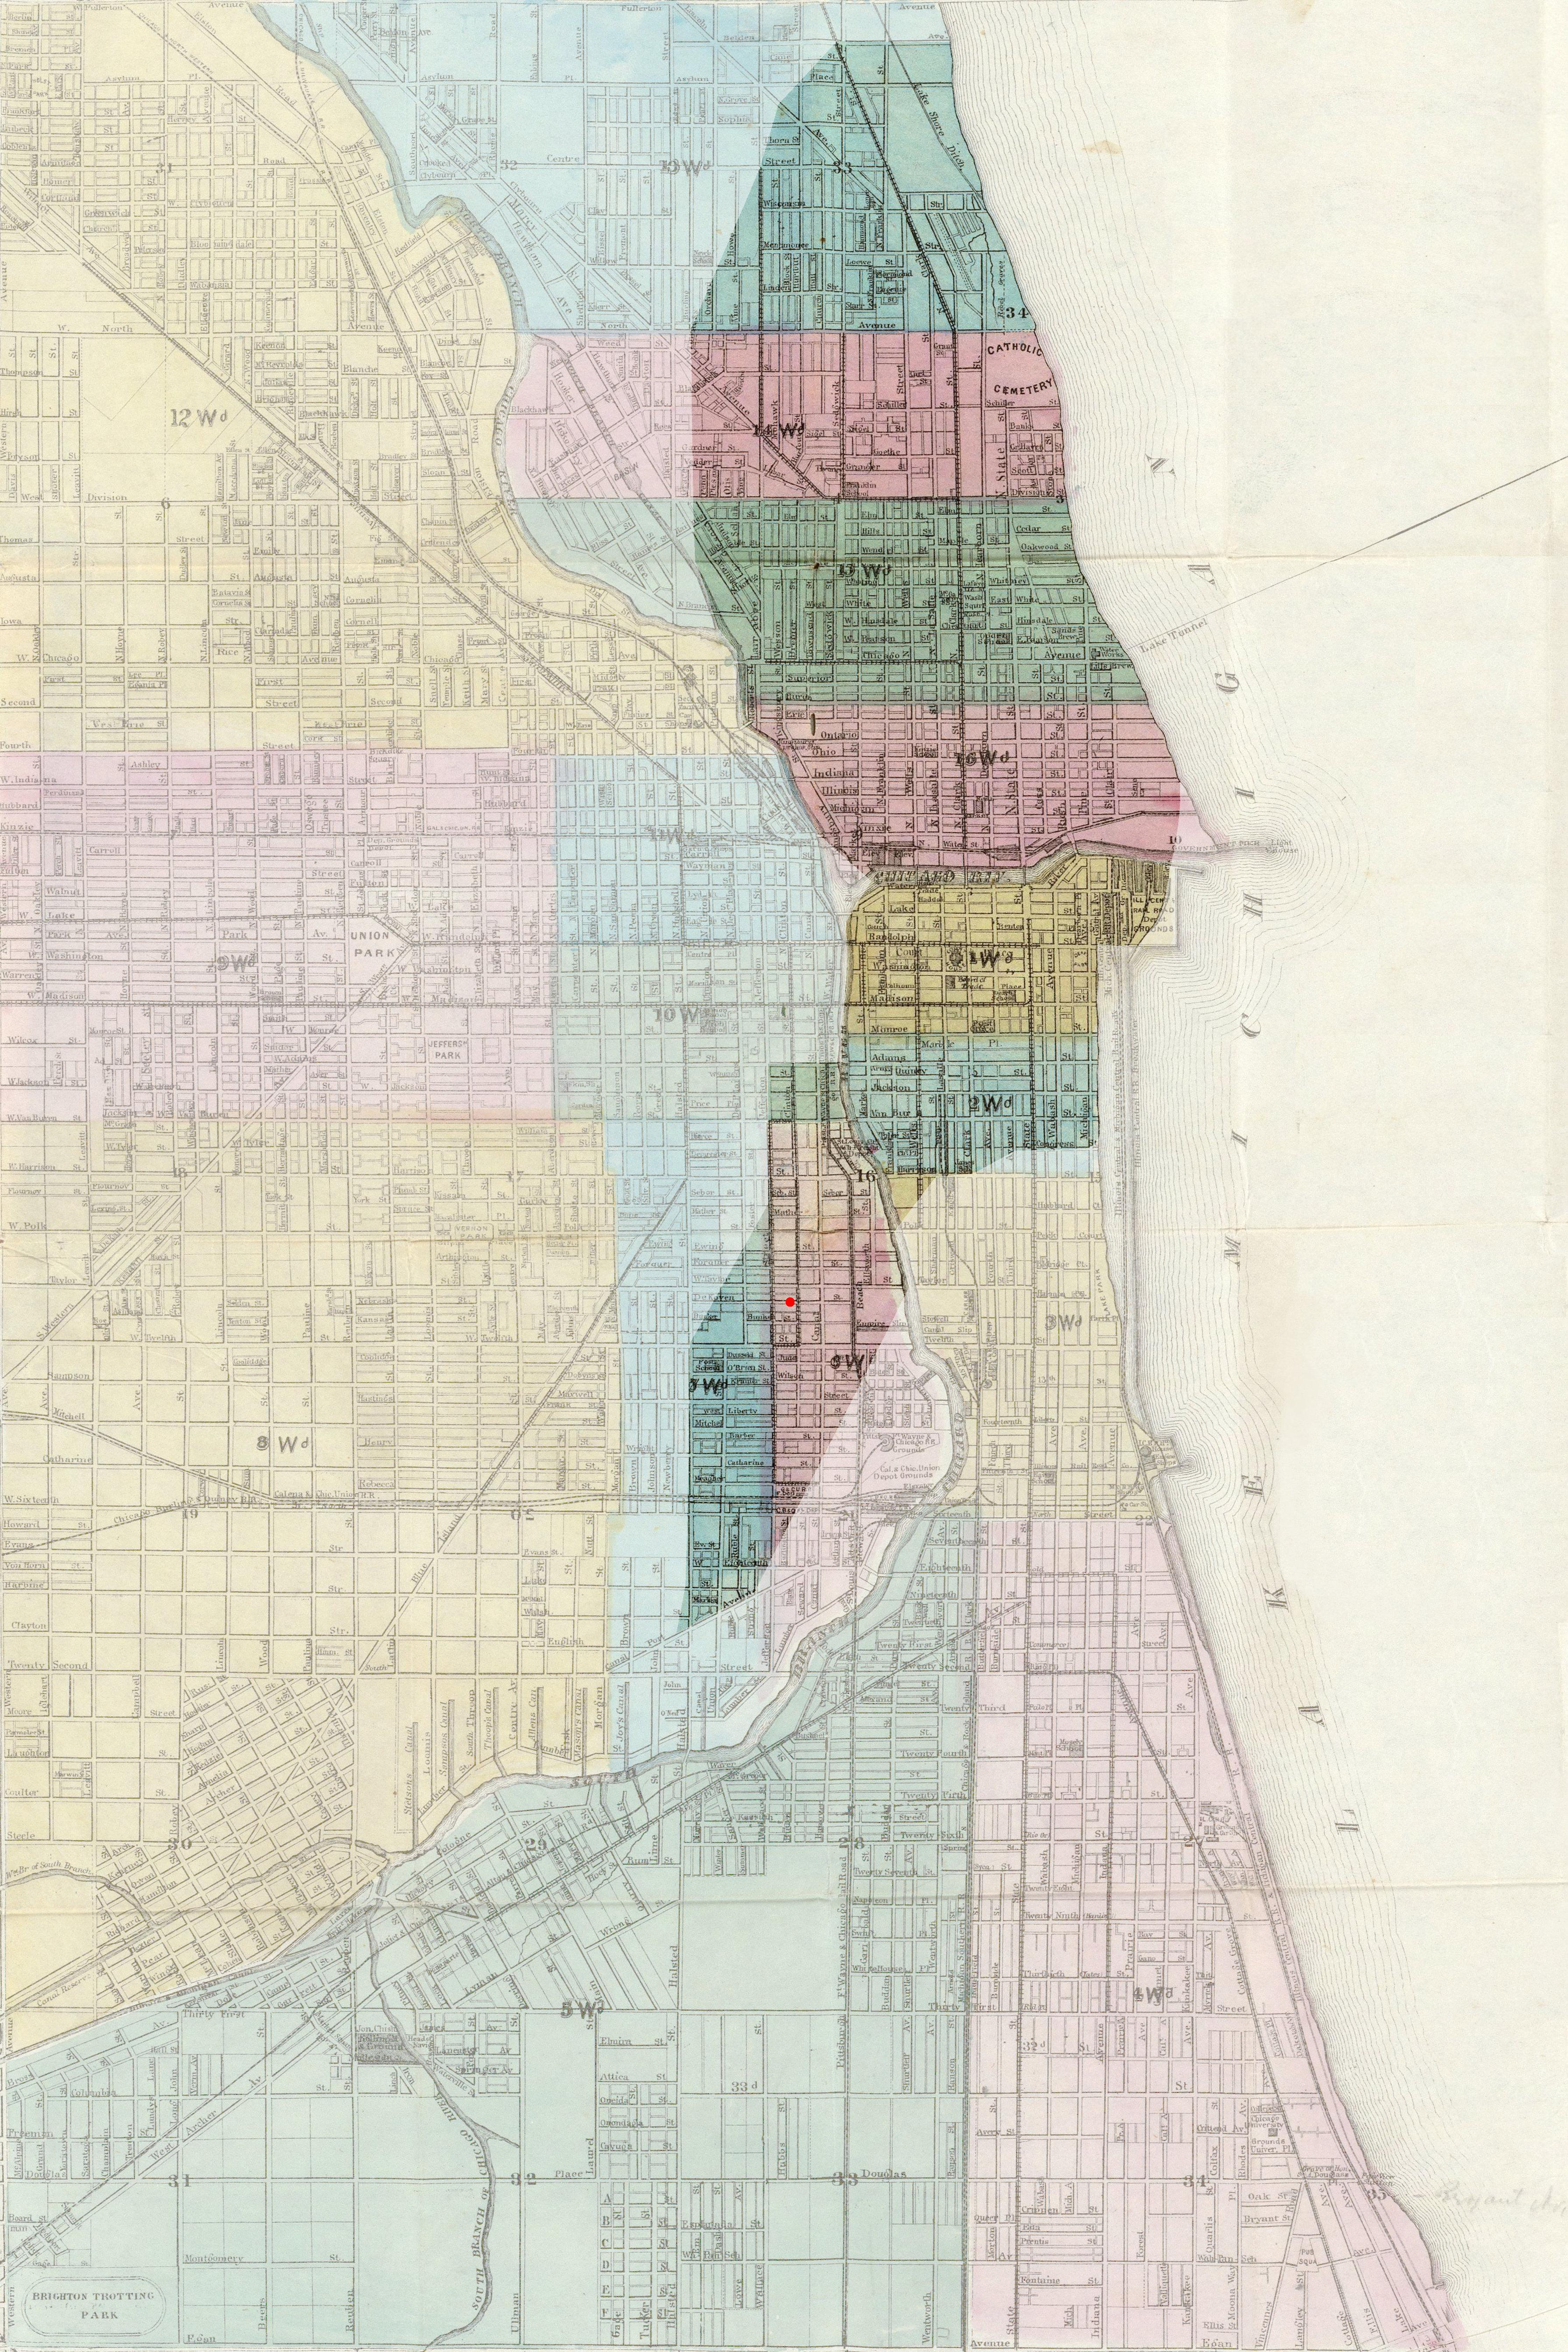
\includegraphics[width=\textwidth,height=0.8\textheight,keepaspectratio=true]{chicago_fire_area}
  \end{center}
\end{frame}

\begin{frame}
  \Large{http://labs.enigma.io/smoke-signals/}
\end{frame}

\begin{frame}
  \frametitle{Surprisingly simple model\dots with mediocre performance}
  \begin{center}
    \includegraphics[width=\textwidth,height=0.8\textheight,keepaspectratio=true]{smoke-alarm-risk/figure/train-model-1}
  \end{center}
\end{frame}

\begin{frame}
  \frametitle{Correlations with smoke detector p/a}
  \begin{columns}
    \begin{column}{0.5\textwidth}
      \includegraphics[width=\textwidth,height=0.8\textheight,keepaspectratio=true]{smoke-alarm-risk/figure/explore-correlations-1-1}
    \end{column}
    \begin{column}{0.5\textwidth}
      \includegraphics[width=\textwidth,height=0.8\textheight,keepaspectratio=true]{smoke-alarm-risk/figure/explore-correlations-1-2}
    \end{column}
  \end{columns}
\end{frame}

\begin{frame}
  \frametitle{Correlations with smoke detector p/a}
  \begin{columns}
    \begin{column}{0.5\textwidth}
      \includegraphics[width=\textwidth,height=0.8\textheight,keepaspectratio=true]{smoke-alarm-risk/figure/score-metrics-1}
    \end{column}
    \begin{column}{0.5\textwidth}
      \includegraphics[width=\textwidth,height=0.8\textheight,keepaspectratio=true]{smoke-alarm-risk/figure/score-metrics-2}
    \end{column}
  \end{columns}
\end{frame}

\begin{frame}
  \frametitle{Variable importance beind risk factor}
  \begin{center}
    \includegraphics[width=\textwidth,height=0.8\textheight,keepaspectratio=true]{smoke-alarm-risk/figure/var-importance-1}
  \end{center}
\end{frame}

\begin{frame}
  \Large{But what about us?}
\end{frame}

\begin{frame}
  \frametitle{Chicago population size and risk}
  \begin{center}
    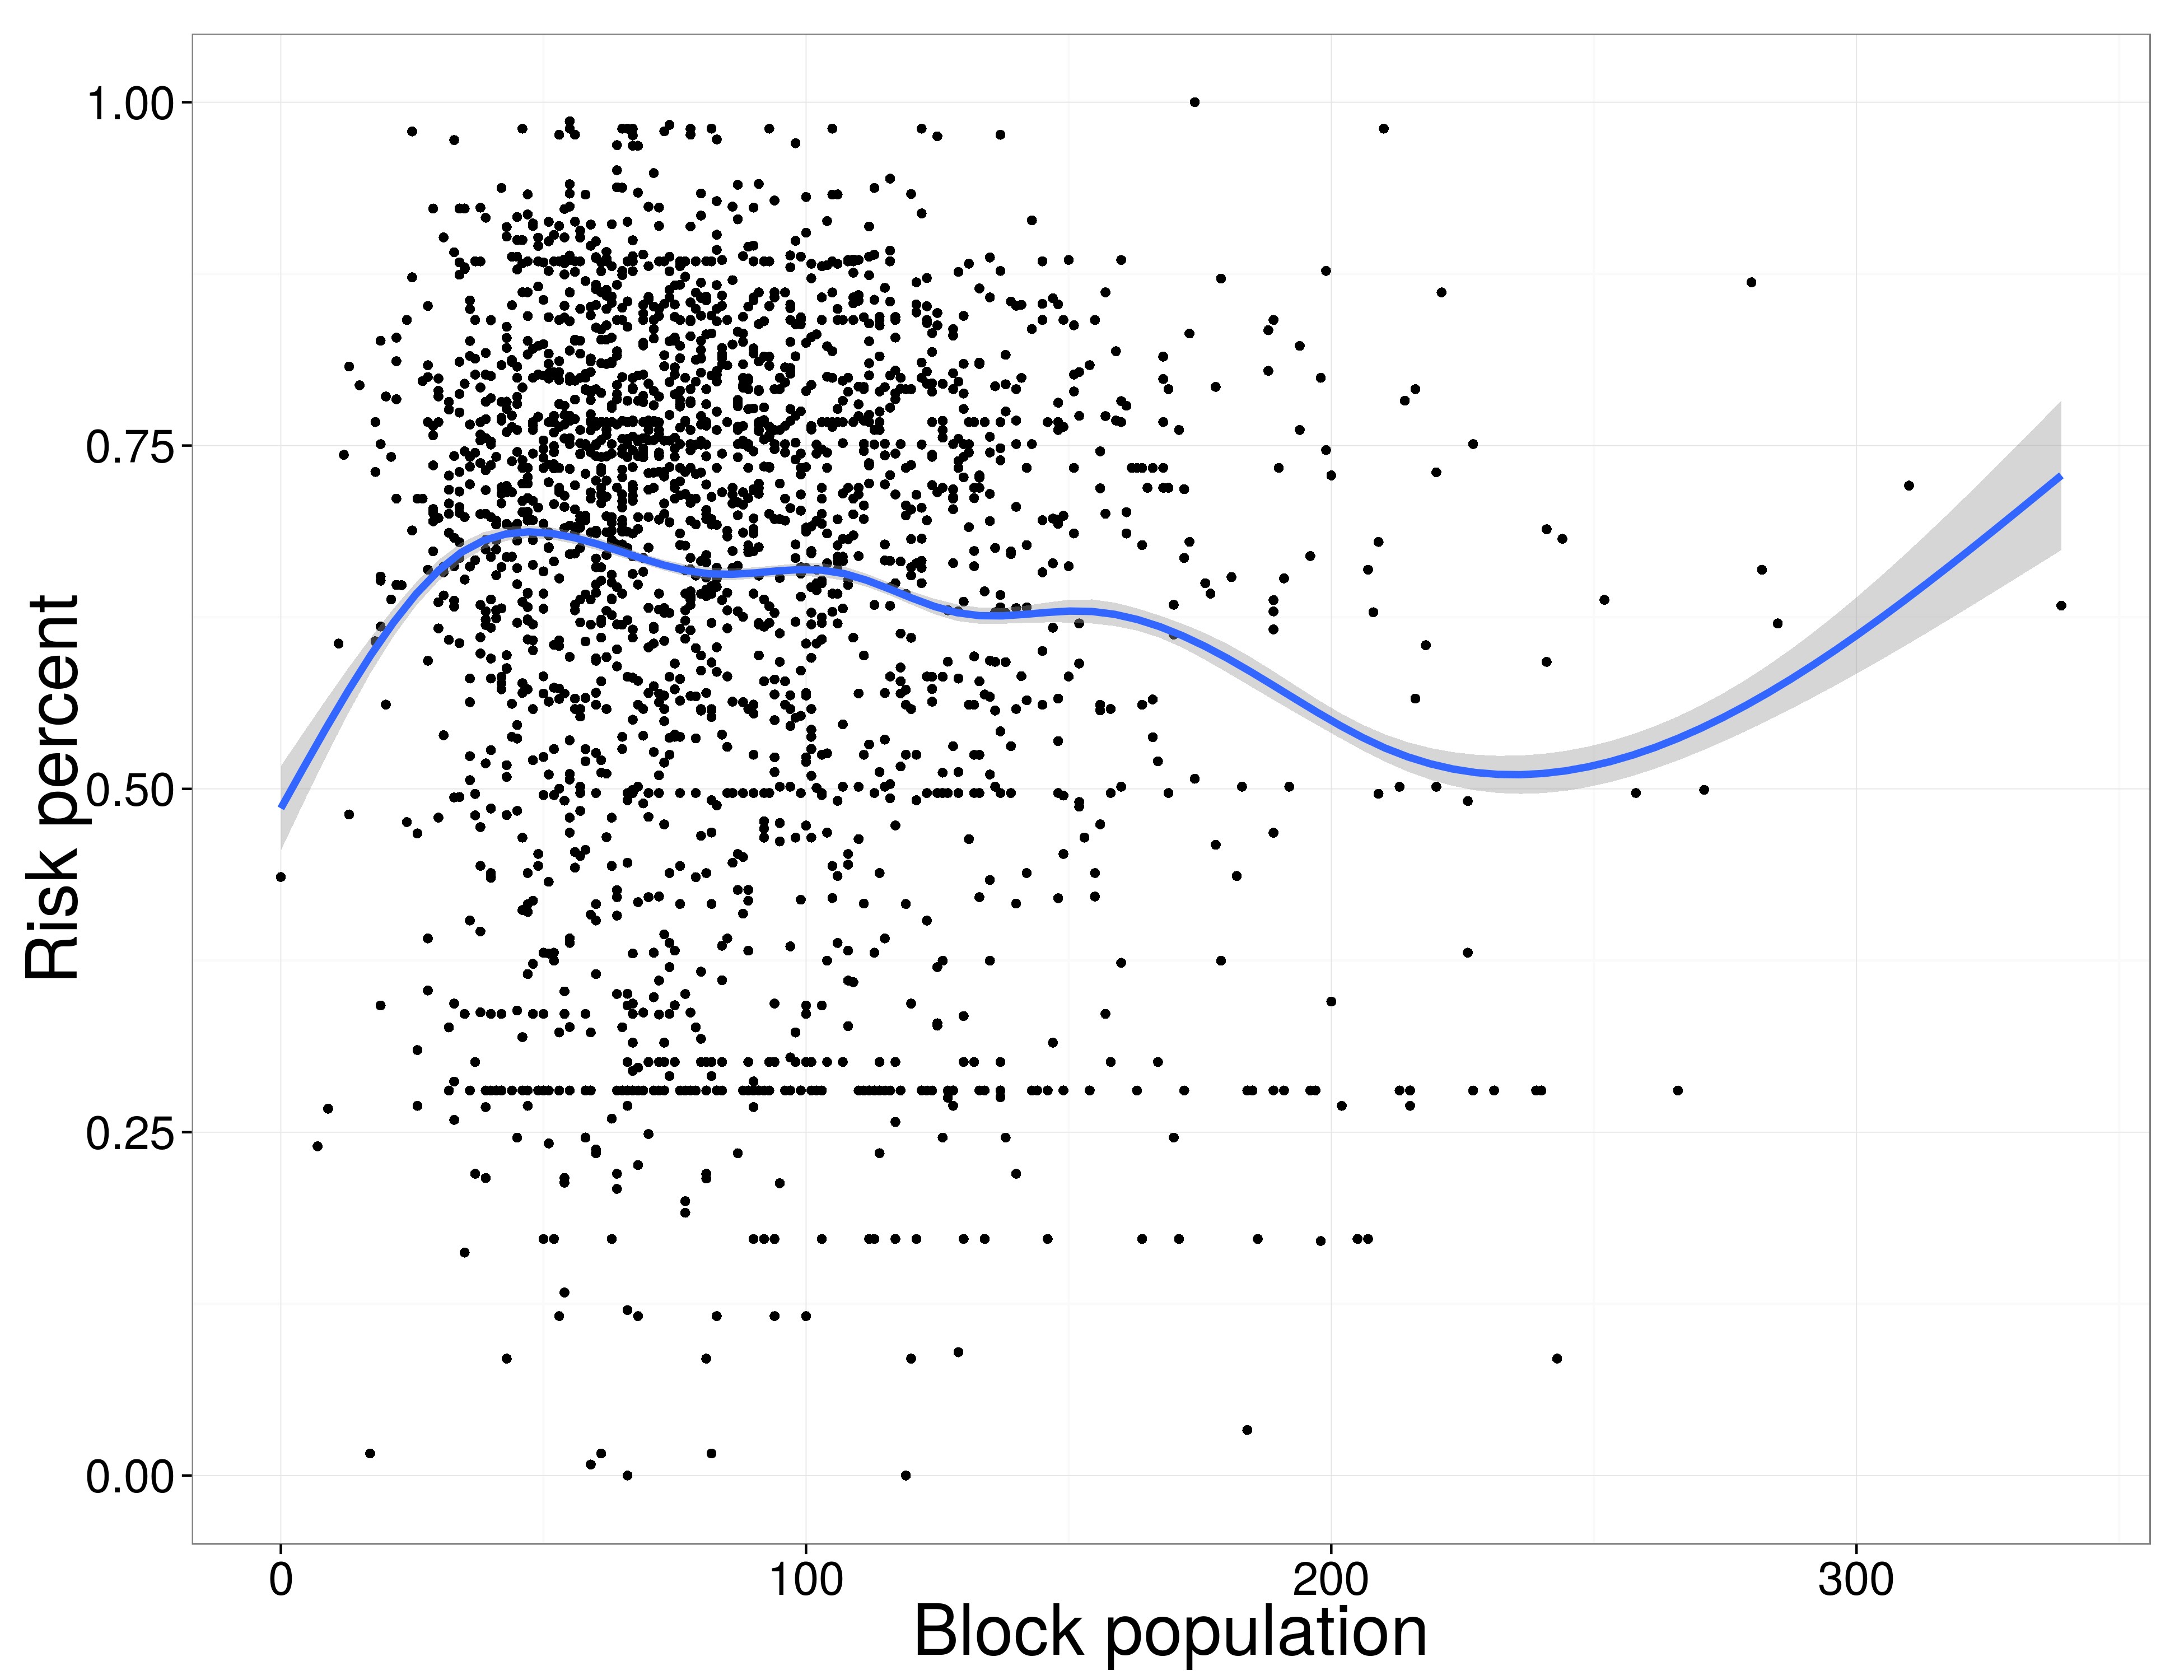
\includegraphics[width=\textwidth,height=0.8\textheight,keepaspectratio=true]{pop_risk}
  \end{center}
\end{frame}

\begin{frame}
  \frametitle{Chicago risk and percent population at risk}
  \begin{center}
    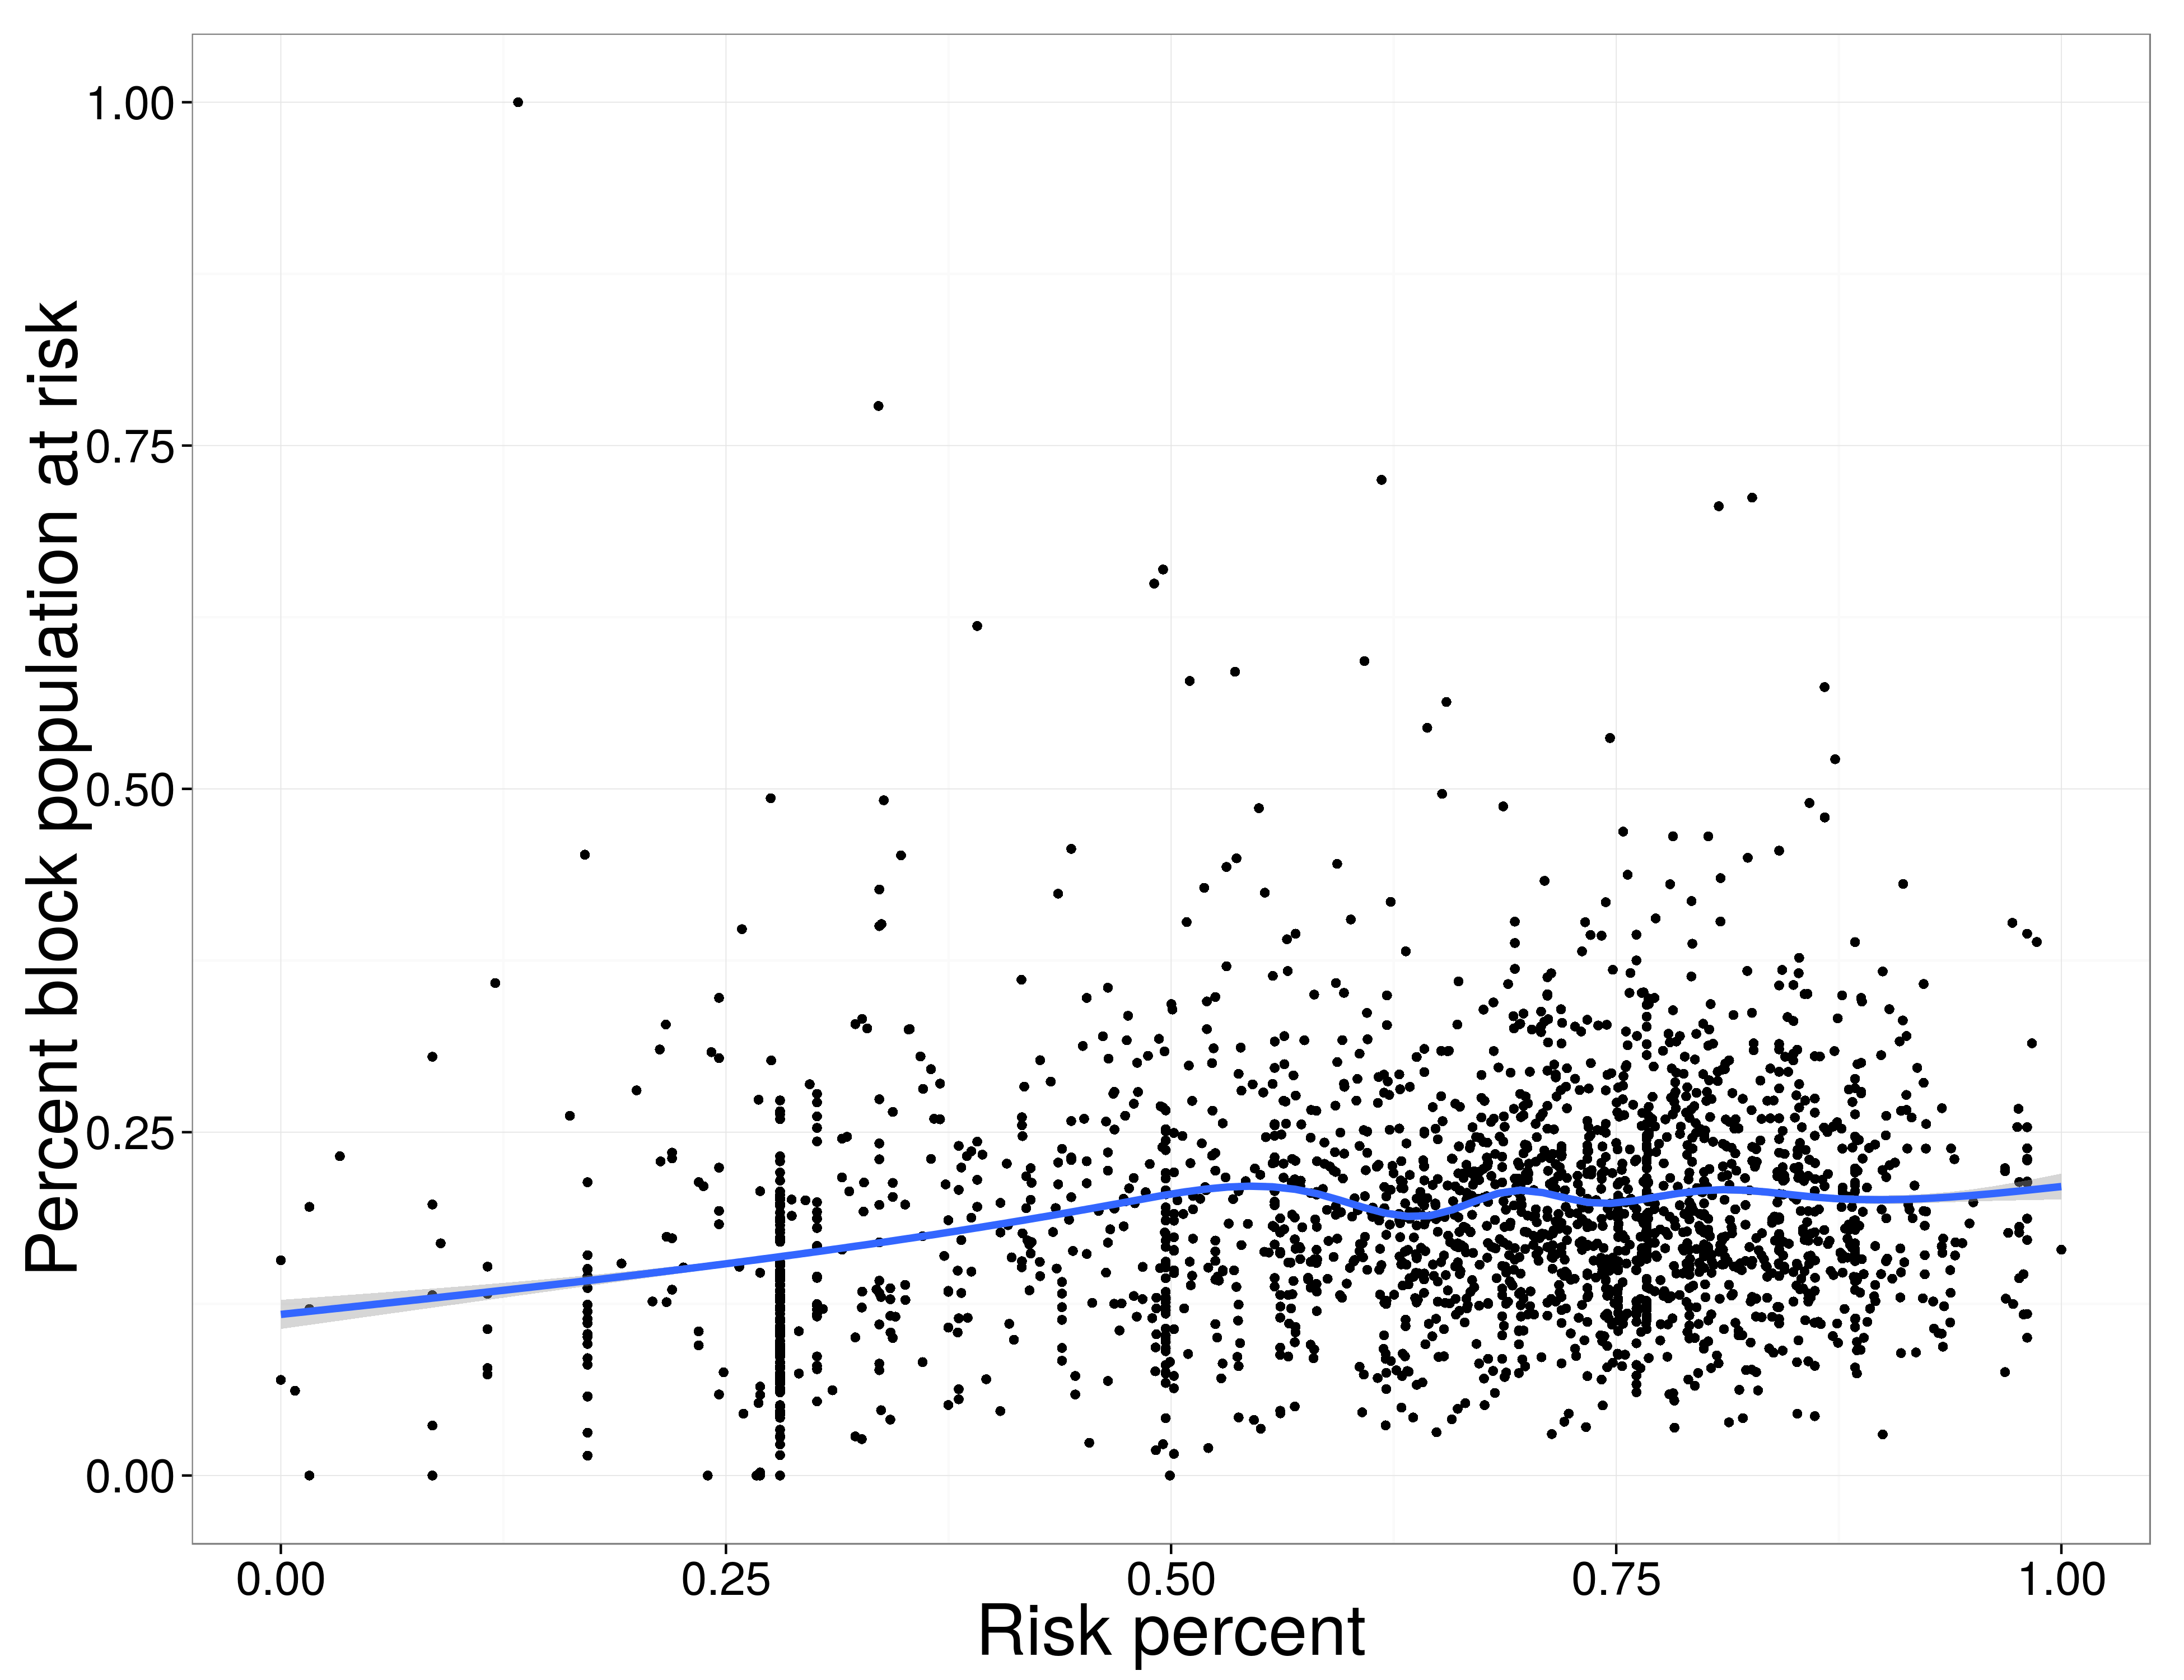
\includegraphics[width=\textwidth,height=0.8\textheight,keepaspectratio=true]{pop_fact}
  \end{center}
\end{frame}

\begin{frame}
  \frametitle{Compared to the rest of Chicago}
  \begin{center}
    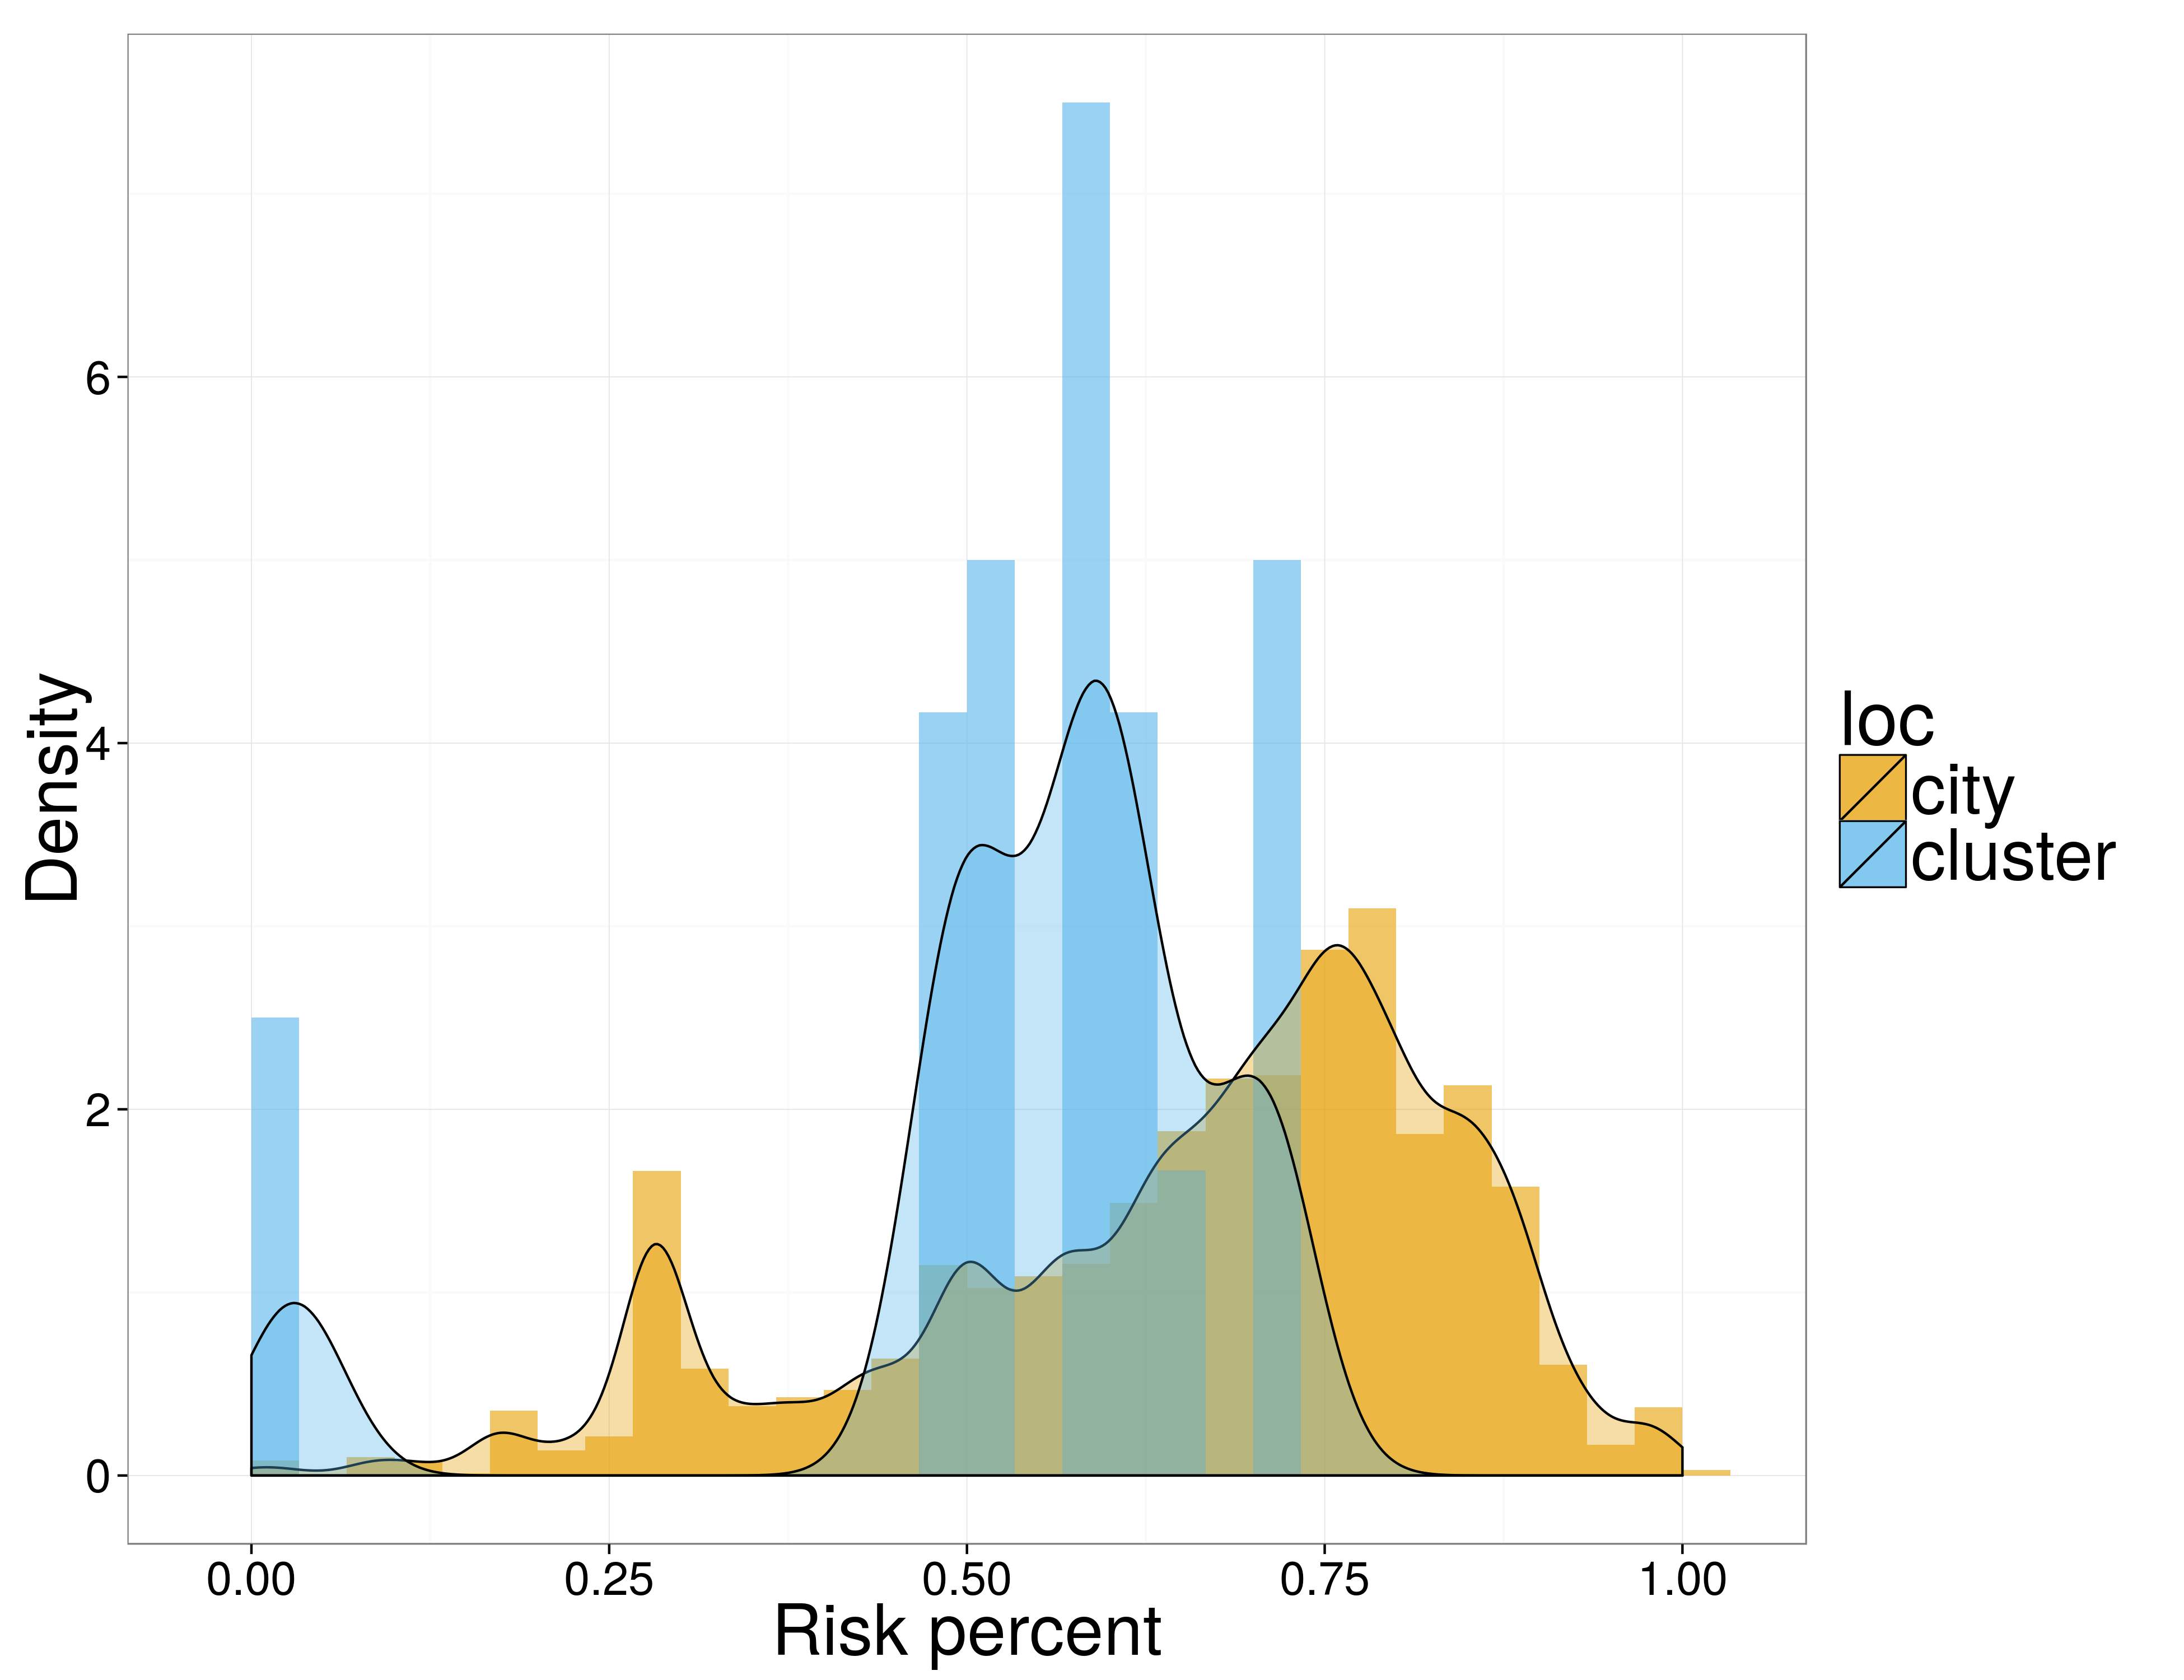
\includegraphics[width=\textwidth,height=0.8\textheight,keepaspectratio=true]{big_risk}
  \end{center}
\end{frame}

\begin{frame}
  \frametitle{Cluster by year}
  \begin{center}
    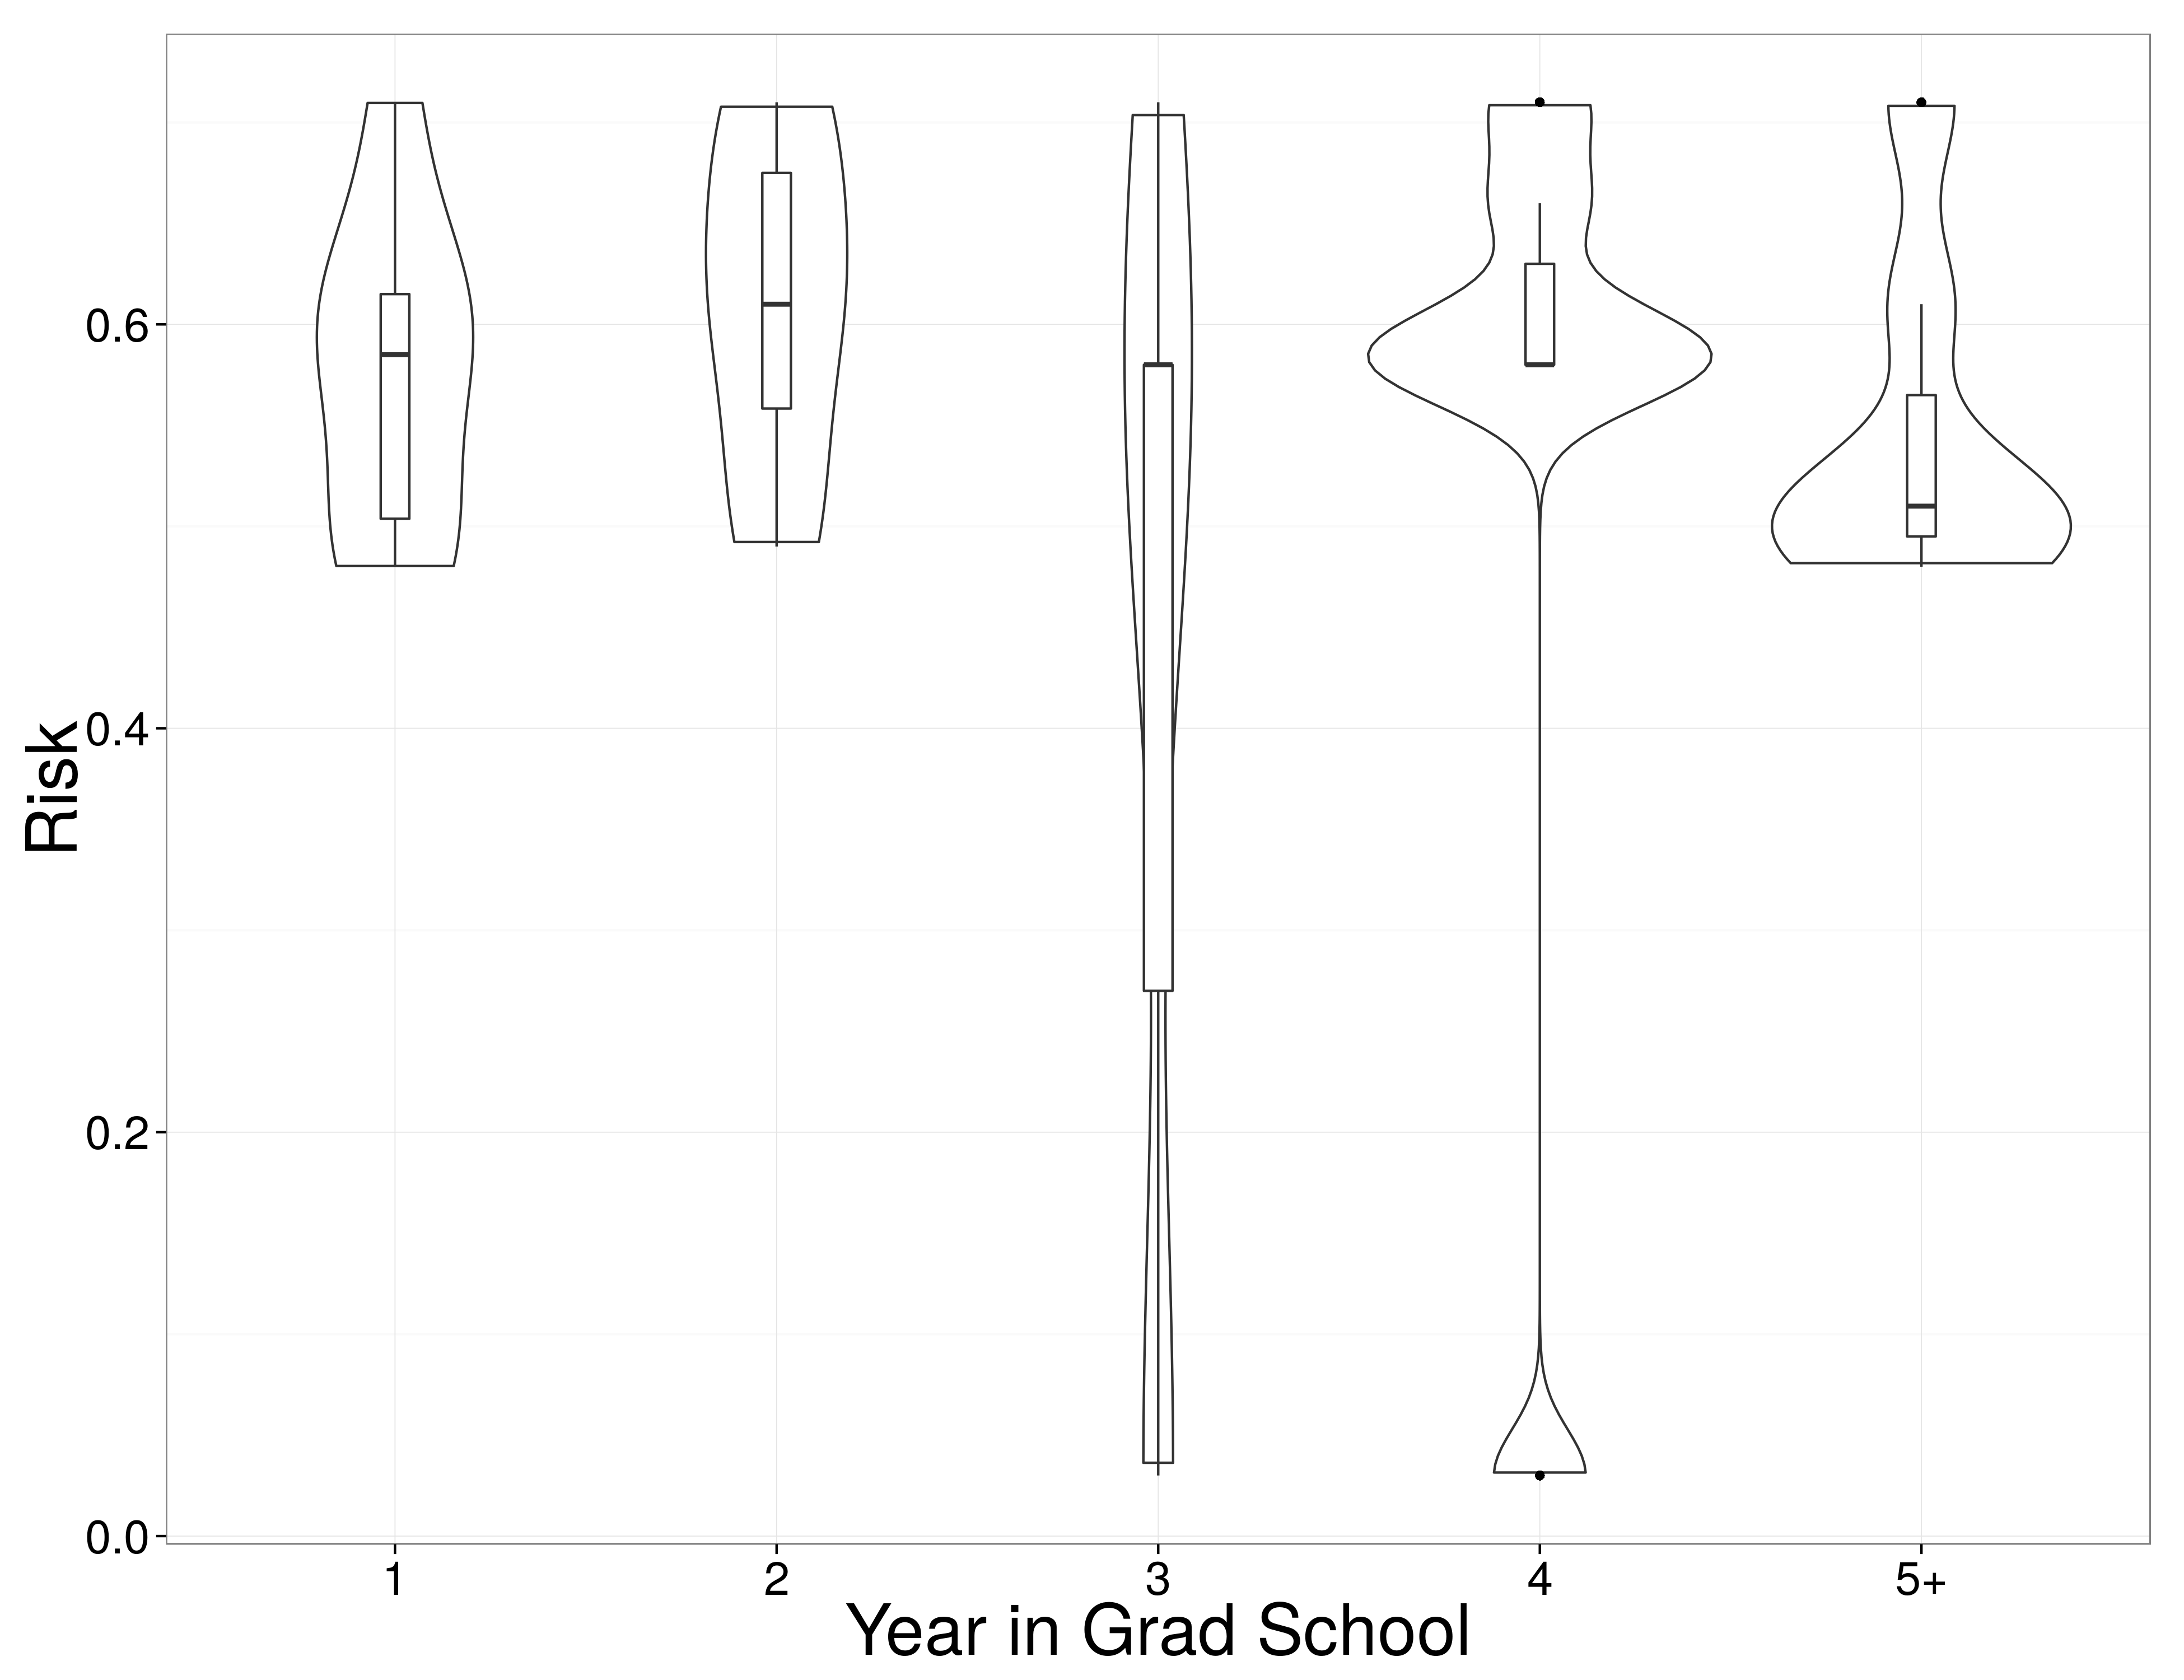
\includegraphics[width=\textwidth,height=0.8\textheight,keepaspectratio=true]{clu_dif}
  \end{center}
\end{frame}

\begin{frame}
  \frametitle{Cluster by ``alarm'' state}
  \begin{center}
    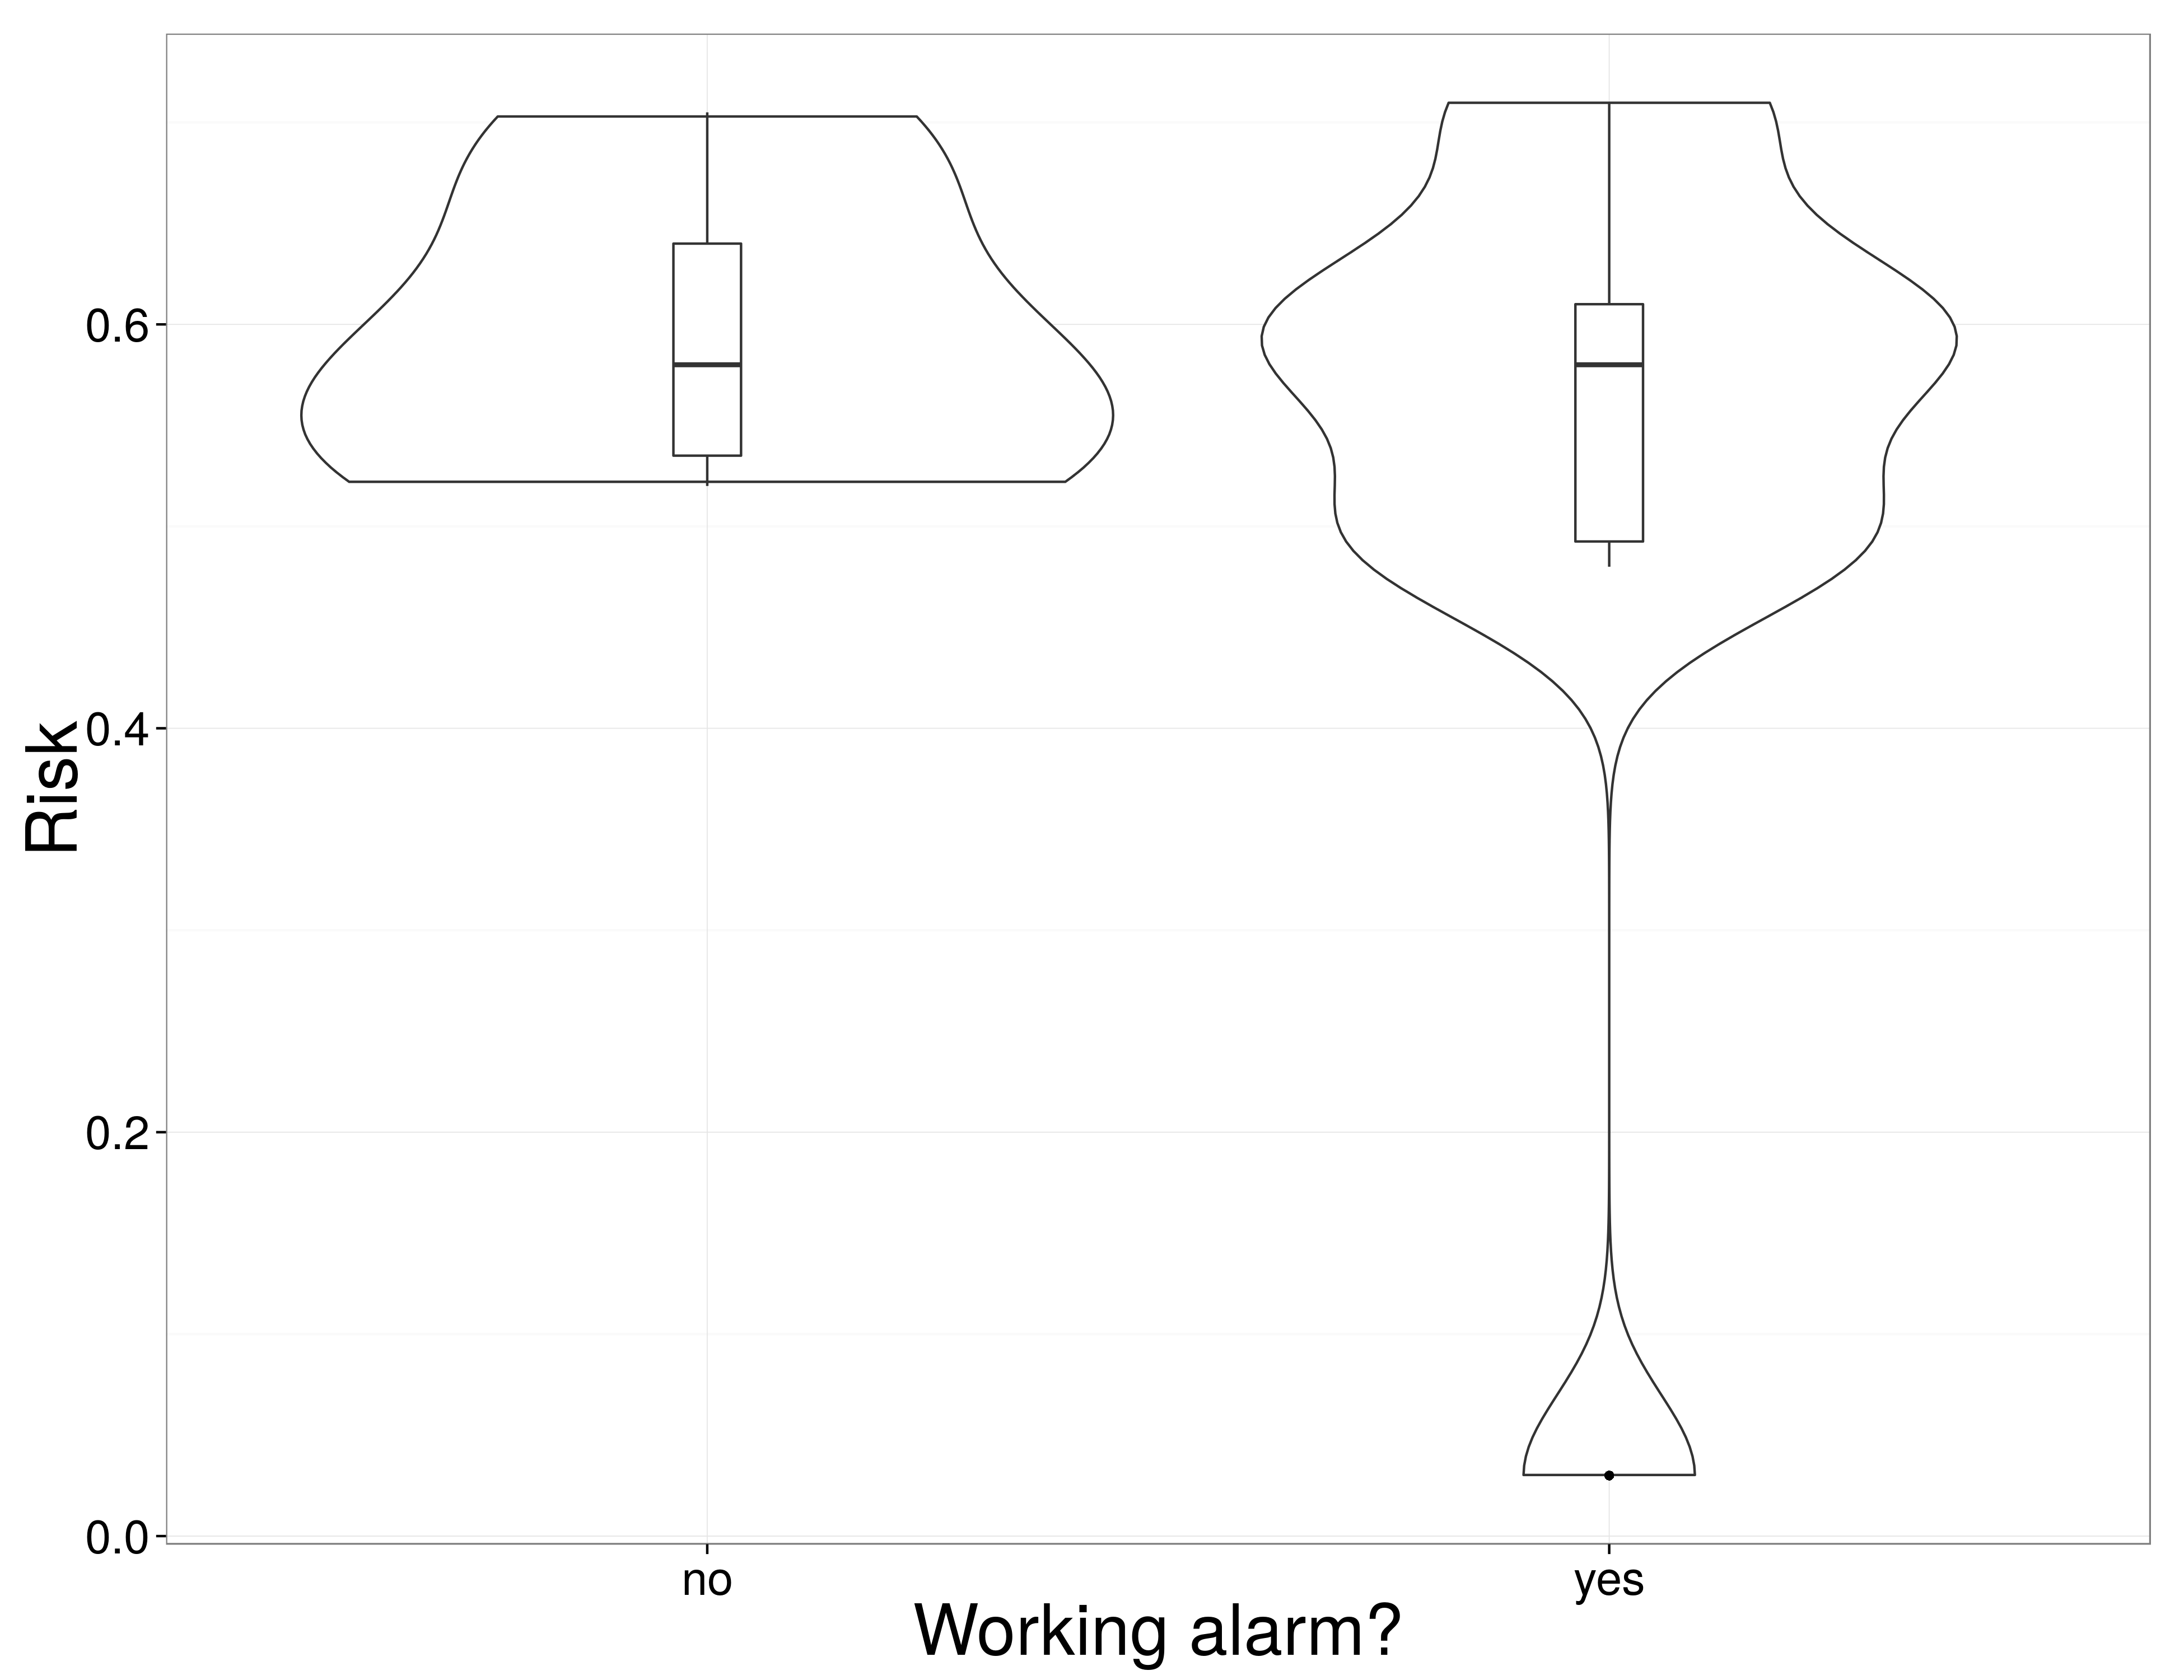
\includegraphics[width=\textwidth,height=0.8\textheight,keepaspectratio=true]{clu_alm}
  \end{center}
\end{frame}

\begin{frame}
  \frametitle{Year by ``alarm'' state}
  \begin{center}
    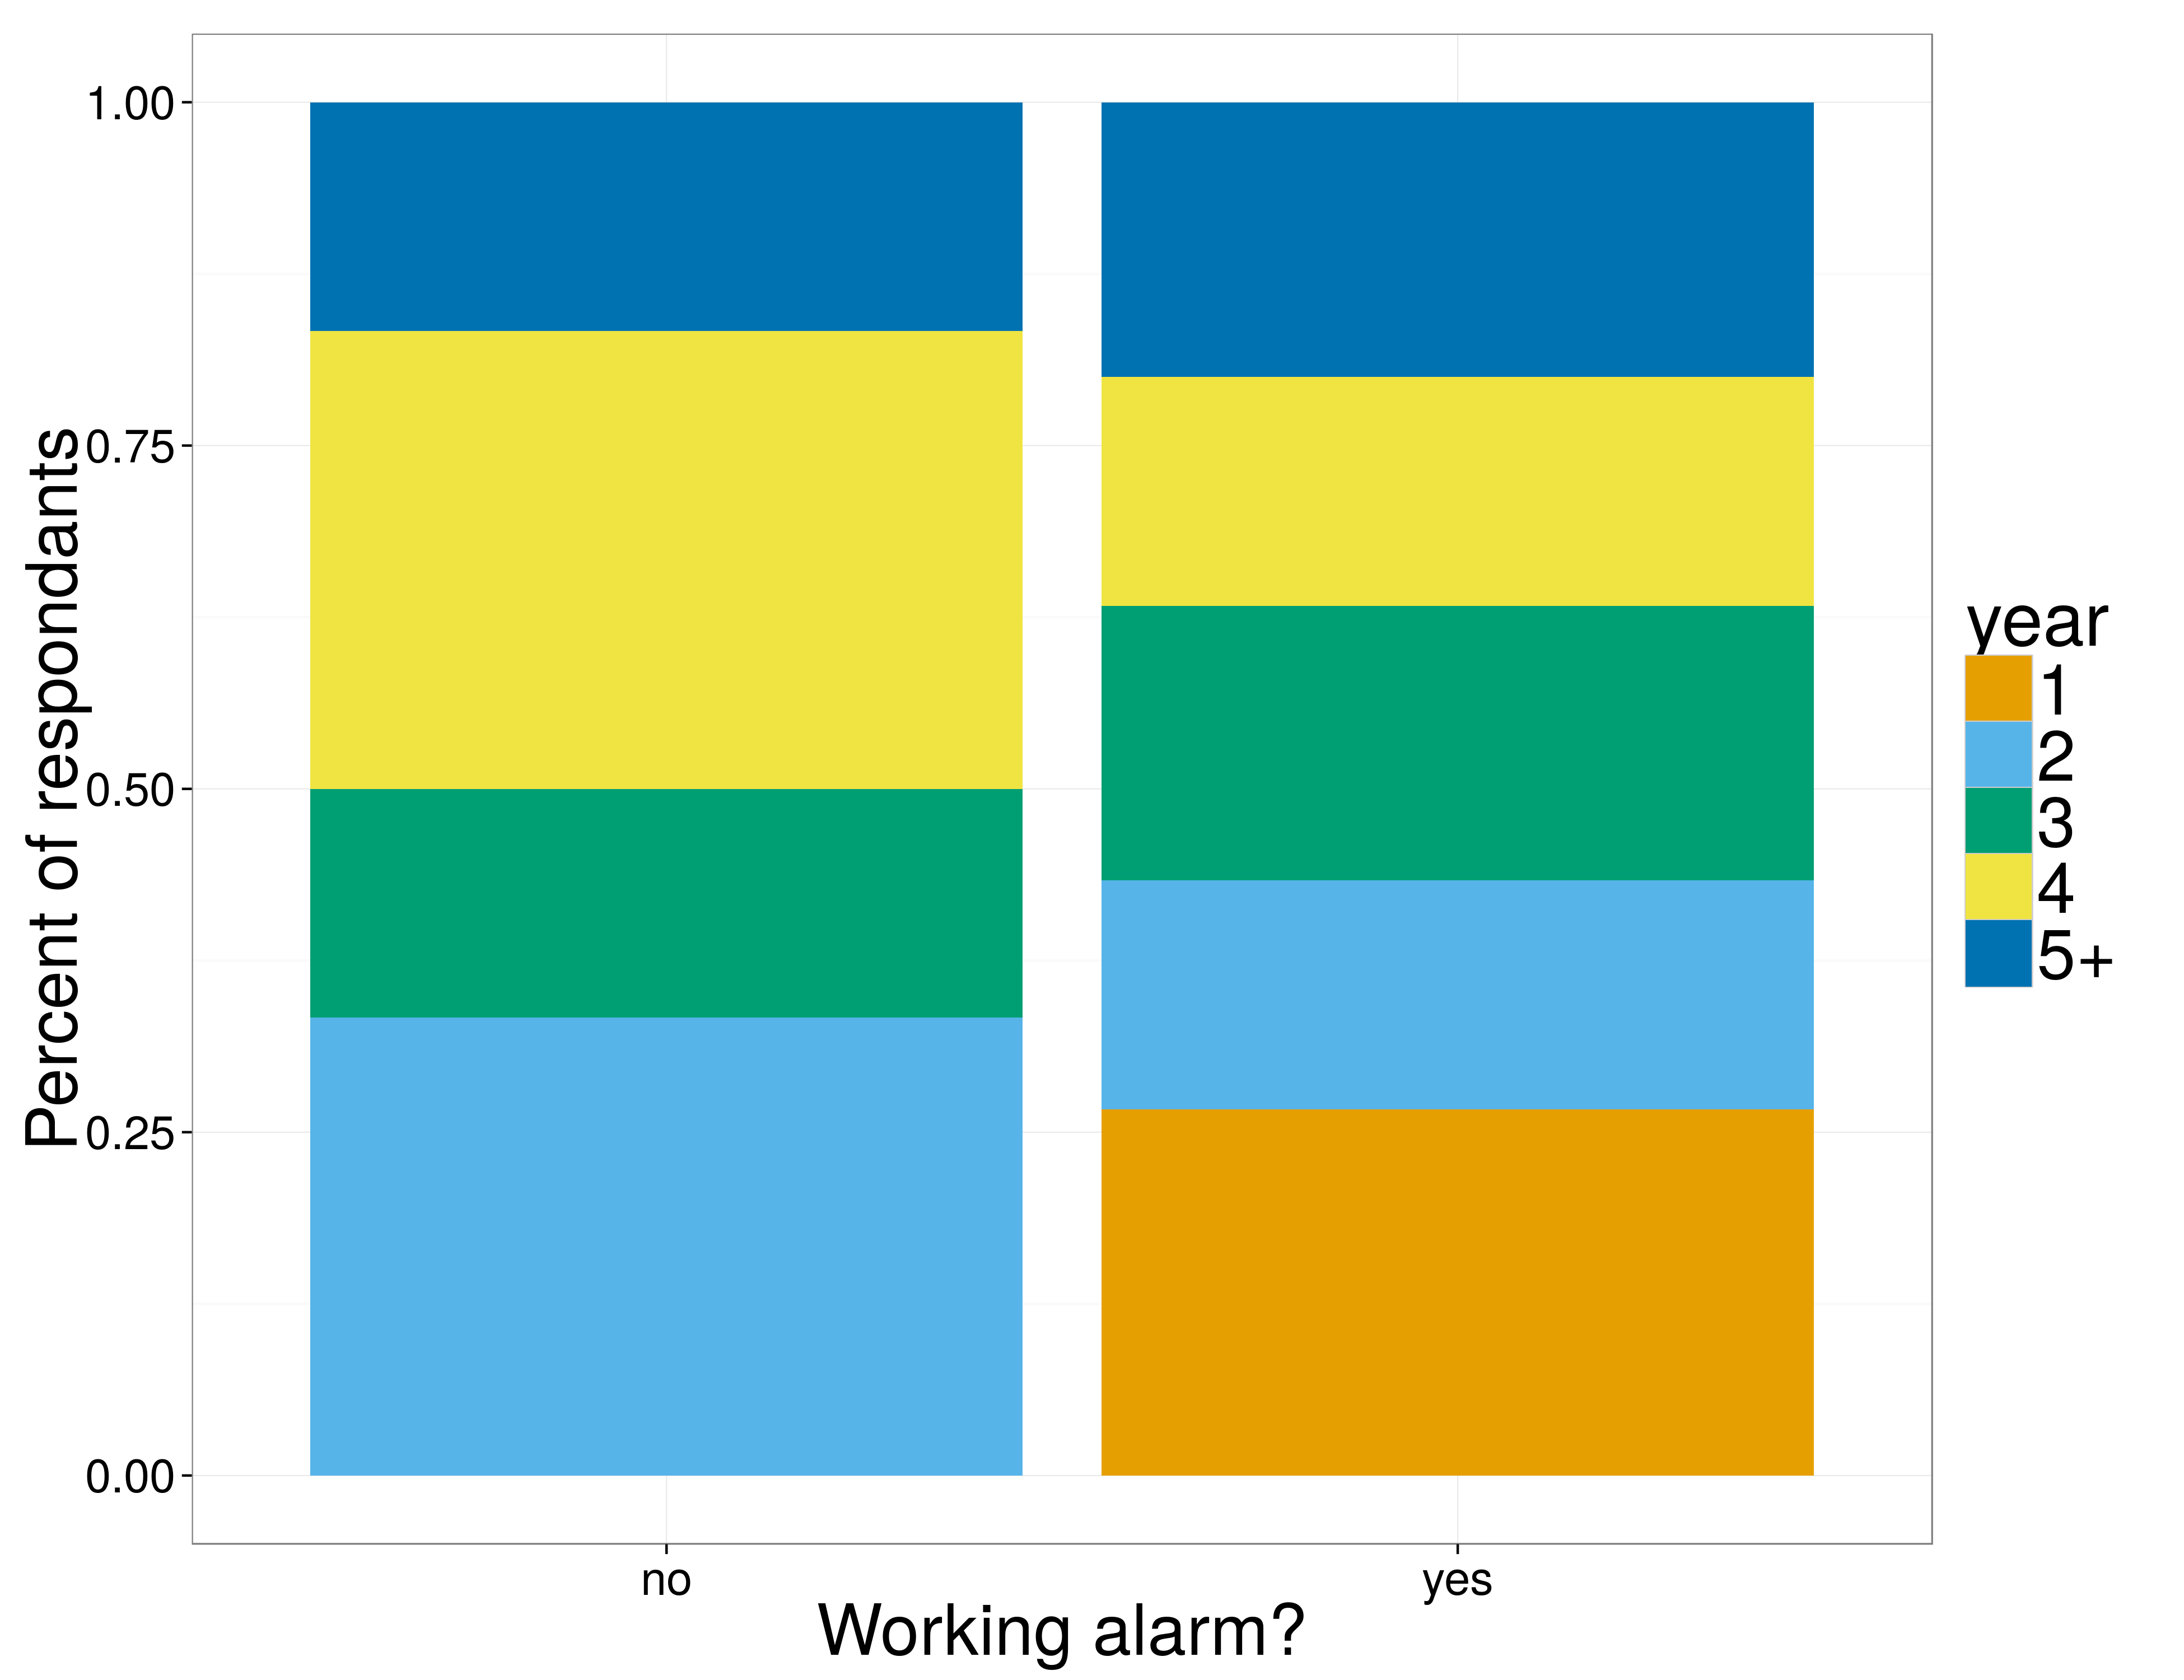
\includegraphics[width=\textwidth,height=0.8\textheight,keepaspectratio=true]{work_alm}
  \end{center}
\end{frame}

\begin{frame}
  \Large{Fire stories}
\end{frame}

\begin{frame}
  \Large{Ermin!}
\end{frame}

\begin{frame}
  \begin{center}
    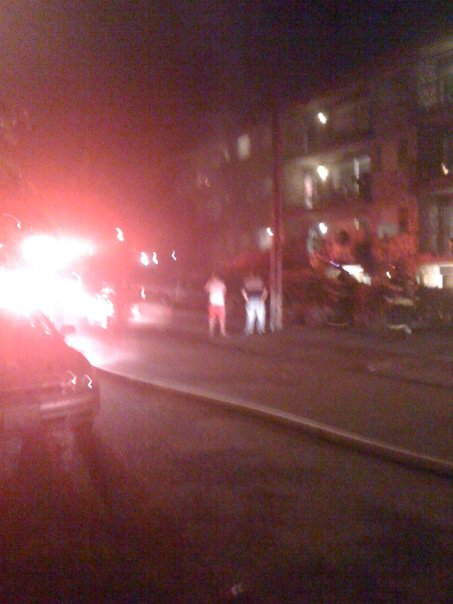
\includegraphics[width=\textwidth,height=0.8\textheight,keepaspectratio=true]{seattle_fire}
  \end{center}
\end{frame}

\begin{frame}
  \begin{center}
    
\includegraphics[width=\textwidth,height=0.8\textheight,keepaspectratio=true]{japan_fire}
  \end{center}
\end{frame}

\end{document}
